\section{Representation of Results}
There are two primary methods to represent the results of multi-person pose
tracking: metric-based evaluation and visual representation.

\subsection{Metric-Based Representation}
The first method uses established metrics to assess the performance of the pose
tracking system. Metrics such as Multiple Object Tracking Accuracy (MOTA) and
mean Average Precision (mAP), as discussed in \cite{andriluka2018posetrack}, can
be employed to evaluate and compare the accuracy of tracking and pose estimation
models.

Figure \ref{fig:mota_map} illustrates these metrics across various video
sequences. The sequences are sorted by average MOTA (left), with pose estimation
results sorted according to the articulation complexity of each sequence
(middle). The right plot visualizes the correlation between mAP and MOTA for
each sequence, highlighting sequences where pose estimation performs well but
tracking still fails. This figure effectively demonstrates how MOTA and mAP can
be used to analyze and compare the performance of pose tracking models under
different conditions.

\begin{figure}[ht!]
    \centering
    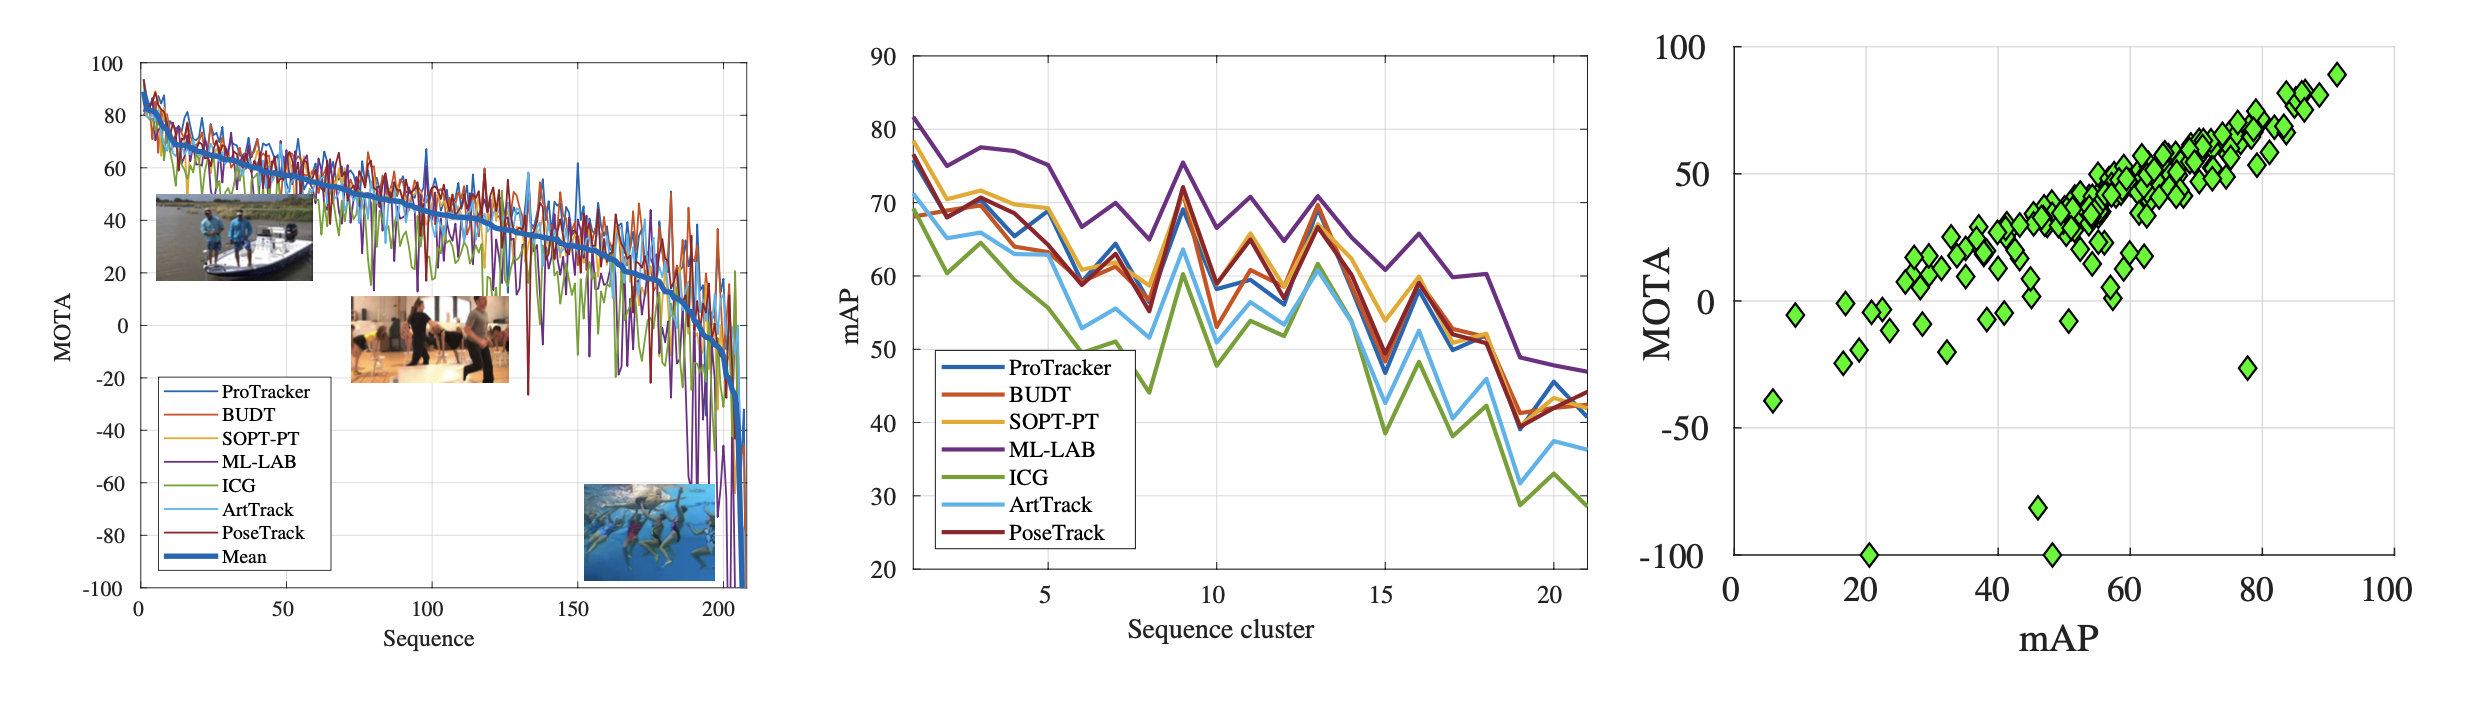
\includegraphics[width=\textwidth]{figs/metrics.png} 
    \caption{Sequences sorted by average MOTA (left). Pose estimation results
    sorted by articulation complexity of the sequence (middle). Correlation
    between mAP and MOTA for each sequence (right). Reproduced from
    \cite{andriluka2018posetrack}.}
    \label{fig:mota_map}
\end{figure}

\subsection{Visual Representation} The second method for representing pose
tracking results is through visualizations \ref{fig:visualizations}. This
approach involves drawing the detected keypoints on each person and connecting
them with lines, creating a stickman-like skeleton. This visual representation
not only shows the positions of the keypoints but also illustrates the
relationships between them, making it easier to interpret the pose of each
person in a scene.

By connecting the keypoints with lines, one can clearly see the structure of the
pose, including the positions of limbs and joints. This visual representation is
particularly useful for quickly assessing the accuracy and quality of the pose
tracking results, as it provides an intuitive way to verify whether the
keypoints have been correctly identified and connected.

\begin{figure}[ht!]
    \centering
    \begin{subfigure}[b]{0.3\textwidth}
        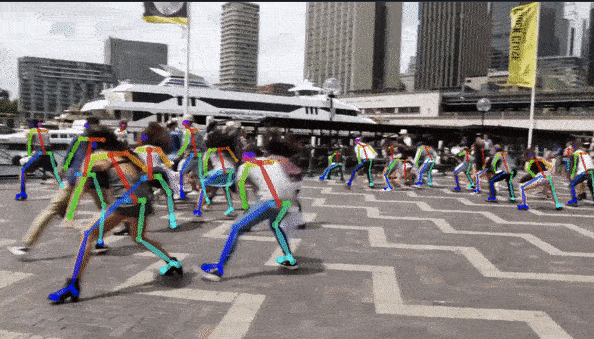
\includegraphics[width=\textwidth]{figs/openpose.png} 
        \caption{From \cite{cao2017realtime}}
        \label{fig:openpose}
    \end{subfigure}
    \hfill
    \begin{subfigure}[b]{0.3\textwidth}
        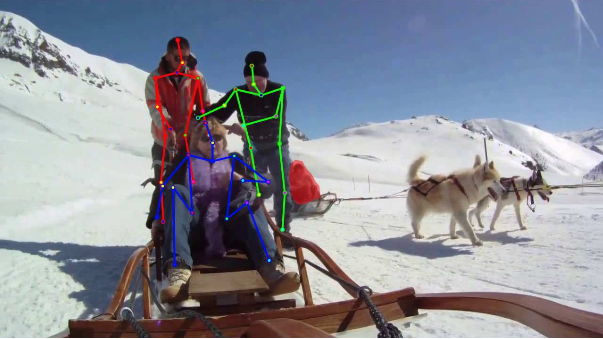
\includegraphics[width=\textwidth]{figs/posetrack.png}
        \caption{From \cite{andriluka2018posetrack}}
        \label{fig:posetrack}
    \end{subfigure}
    \hfill
    \begin{subfigure}[b]{0.3\textwidth}
        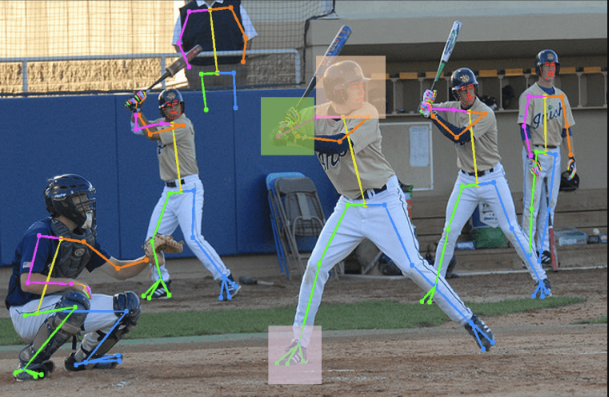
\includegraphics[width=\textwidth]{figs/coco-wholebody.png}
        \caption{From \cite{jin2020whole}}
        \label{fig:coco-wholebody}
    \end{subfigure}
    \begin{subfigure}[b]{0.3\textwidth}
        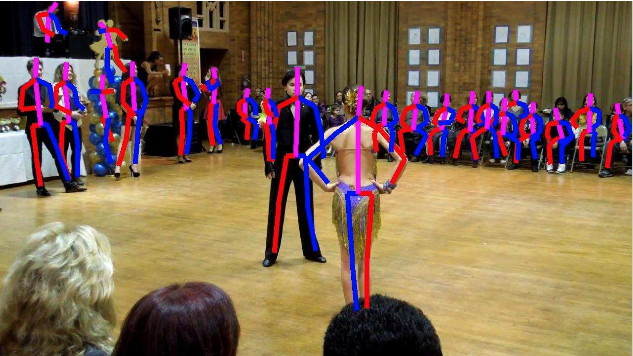
\includegraphics[width=\textwidth]{figs/fang-rmpe.png}
        \caption{From \cite{fang2017rmpe}}
        \label{fig:fang-rmpe}
    \end{subfigure}
    \begin{subfigure}[b]{0.3\textwidth}
        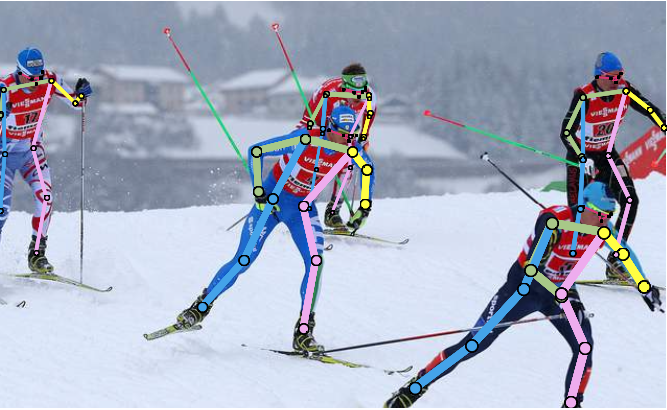
\includegraphics[width=\textwidth]{figs/sundeep.png}
        \caption{From \cite{sun2019deep}}
        \label{fig:sundeep}
    \end{subfigure}
    \begin{subfigure}[b]{0.3\textwidth}
        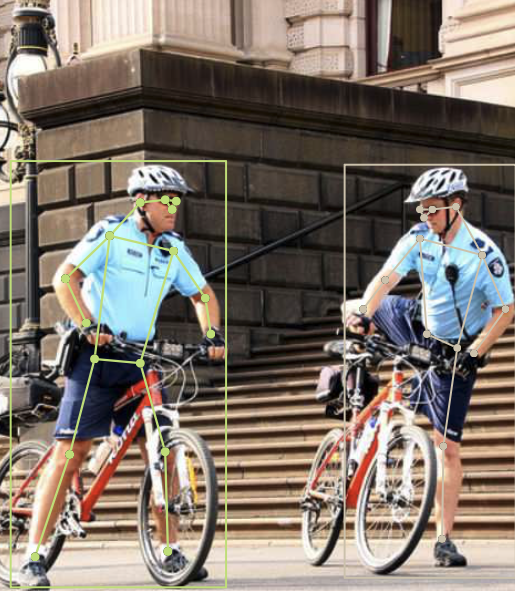
\includegraphics[width=\textwidth]{figs/papandreou.png}
        \caption{From \cite{Papandreou_2017_CVPR}}
        \label{fig:papandreou}
    \end{subfigure}
    \begin{subfigure}[b]{0.3\textwidth}
        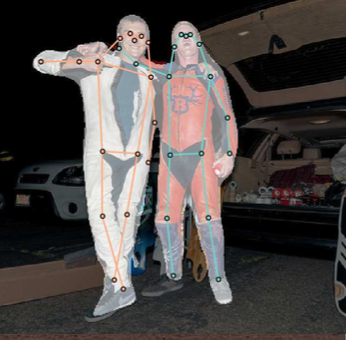
\includegraphics[width=\textwidth]{figs/kokabas.png}
        \caption{From \cite{Kocabas_2018_ECCV}}
        \label{fig:kocabas}
    \end{subfigure}
    \begin{subfigure}[b]{0.3\textwidth}
        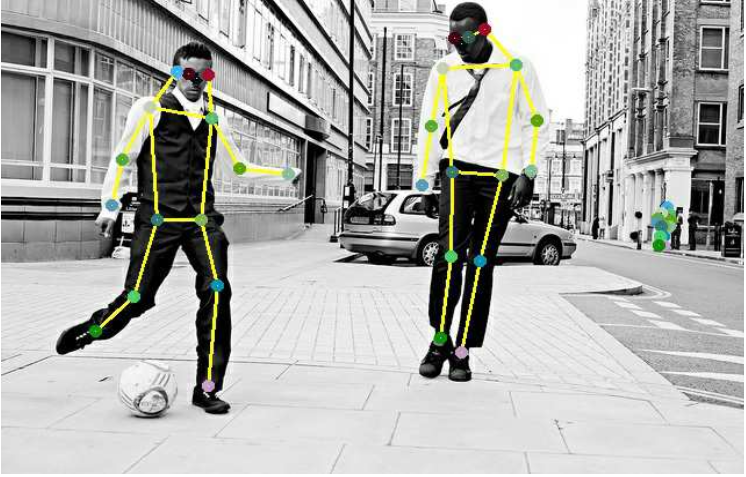
\includegraphics[width=\textwidth]{figs/chen.png}
        \caption{From \cite{chen2018cascaded}}
        \label{fig:chen}
    \end{subfigure}
    \begin{subfigure}[b]{0.3\textwidth}
        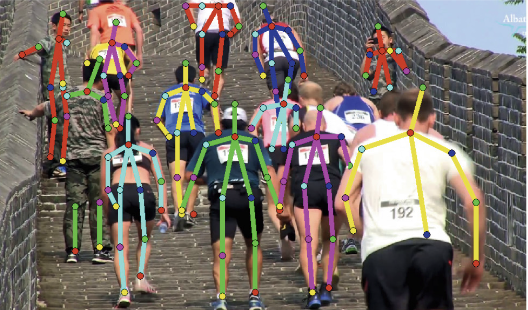
\includegraphics[width=\textwidth]{figs/deeper.png}
        \caption{From \cite{insafutdinov2016deepercut}}
        \label{fig:deeper}
    \end{subfigure}
    \caption{Visual representation from a number of different multi person pose estimation papers}
    \label{fig:visualizations}
\end{figure}

Both metric-based and visual representations are essential for thoroughly
evaluating and demonstrating the effectiveness of multi-person pose tracking
systems. While metrics provide a quantitative assessment, visualizations offer
an immediate, interpretable view of the results, making them complementary tools
in pose tracking analysis.
